\documentclass[12pt,a4paper,twoside]{article}
\usepackage[ngerman]{babel}
\usepackage{amsmath}
\usepackage{amssymb}
\usepackage{graphicx}
\usepackage[utf8]{inputenc}
\usepackage[numbers,round]{natbib}
\usepackage{abschlussarbeit}
\usepackage{hyperref}
\usepackage{mathtools}
\usepackage{dsfont}
%\usepackage{ulem}
\usepackage{color}
\usepackage{enumerate}
%\usepackage{cite}
%\usepackage{natbib}
\usepackage{verbatim}
\setlength{\voffset}{-28.4mm}
\setlength{\hoffset}{-1in}
\setlength{\topmargin}{20mm}
\setlength{\oddsidemargin}{25mm}
\setlength{\evensidemargin}{25mm}
\setlength{\textwidth}{160mm}

\setlength{\parindent}{0pt}

\setlength{\textheight}{235mm}
\setlength{\footskip}{20mm}
\setlength{\headsep}{50pt}
\setlength{\headheight}{0pt}

\pagestyle{headings}
\bibliographystyle{plaindin}

\usepackage[tableposition=top]{caption}
\captionsetup{font={footnotesize}}

\newtheorem{Satz}{Satz}[section]
% Ein sog. "Theorem" mit Abkuerzung "Satz" (das erste "Satz")
% Das zweite "Satz" bezeichnet den Namen des Theorems. (z.B. "Satz x.y" erscheint im TeX-File).
% [chapter] regelt die Numerierung der Saetze, in diesem Fall werden die Saetze pro Kapitel fortlaufend numeriert.

\newtheorem{Korollar}[Satz]{Korollar}
% Hier haben wir ein "Theorem" mit Abkuerzung "Korollar", welches im Tex-File als "Korollar" erscheint und in die "Theorem"-Nummerierung
% fortlaufend eingebunden wird (das "[Theorem]" bewirkt dies).
\newtheorem{Proposition}[Satz]{Proposition}
% Abkuerzung ist "Proposition", Name ist "Proposition", wird in "Theorem"-Nummerierung eingebunden.
%Lemma, ebenfalls in "Theorem"-Nummerierung eingebunden
\newtheorem{Lemma}[Satz]{Lemma}
%Definition, ebenfalls in "Theorem"-Nummerierung eingebunden
\newtheorem{Definition}[Satz]{Definition}
%Beispiel, ohne Nummerierung
\newtheorem{Beispiel}{Beispiel}
\newtheorem{Bemerkung}{Bemerkung}
\newtheorem{Beweis}{Beweis}

%Annahme, nach Kapiteln nummeriert
\newtheorem{Annahme}{Annahme}[section]
% Labelnummerierung in 'roemisch'.
\renewcommand{\labelenumi}{(\roman{enumi})}


\begin{document}
\pagestyle{empty}
%%%% Titelseite
\begin{titlepage}
\begin{center}

\includegraphics{TUMblau.png}\\[3mm]
\sf
{\Large
  Technische Universit"at M"unchen\\[5mm]
  Fakult"at f"ur Mathematik\\[8mm]
}
\normalsize

\includegraphics{MA_Web.png}\\[15mm]

Bachelor-Arbeit\\[15mm]

{\LARGE
Qualitativer Vergleich diverser Methoden zur Matrixrekonstruktion im Kontext der optimalen Stabilisierung des inversen Pendels
}
\bigskip

\normalsize

Markus Stachl
\end{center}
\vspace*{75mm}

Aufgabensteller: Prof. Dr. Oliver Junge
\medskip

Betreuer: Prof. Dr. Oliver Junge
\medskip

Abgabetermin: ...

\end{titlepage}
%%%% Erklaerung - Unterschrift nicht vergessen!

\vspace*{150mm}

Ich erkl"are hiermit, dass ich die Bachelor-Arbeit selbst"andig und nur mit den angegebenen
Hilfsmitteln angefertigt habe.
\bigskip

Garching, den
\newpage
%%%% Zusammenfassung in englischer Sprache
\section*{Summary}
Bei einer in deutscher Sprache verfassten Arbeit muss eine Zusammenfassung in englischer Sprache vorangestellt werden.
Daf"ur ist hier Platz.

\newpage
\tableofcontents
\newpage

%%%% Ab hier beginnt die eigentliche Nummerierung der Seiten
\pagenumbering{arabic}
\pagestyle{headings}

\section{Einführung}
	Seit einigen Jahrzehnten befinden wir uns in einer Gesellschaft, in der wir freien Zugang zu aller Arten von 
	Informationen haben. Durch Wissens-Datenbanken wie Wikipedia wird jedem der Zugriff zu Spezialwissen verschiedenster Themen ermöglicht und jeder Experte kann sein eigenes Spezialwissen inserieren und somit verbreiten.
%	 Durch die Entwicklung von Suchmaschinen wie Google und Yahoo wird der Zugriff auf diese Quellen erleichtert. 
%	Durch den stetigen Upload an Daten steht die Informationstheorie vor einem neuen Problem: how to handle Big Data.
%	Laut einer Studie der \textit{pcwelt} hat die Menschheit bis zum Jahre 2013 über 2 Zettabyte (Zetta = $10^{21}$) Daten produziert und gespeichert.
	\\
	In dem Informationszeitalter, in dem dem sich unsere Gesellschaft derzeit befindet, liegt das Augenmerk nicht 
	mehr in der Informationsbeschaffung, sondern in der Speicherung dieser Informationen und der Erleichterung des 
	Zugriffs auf diese. \\
	Leider nimmt die Leistungsfähigkeit der Rechner nicht in dem selben Maße zu wie die Menge an Daten. Aus diesem 
	Grund ist es notwendig, durch die Untersuchung einer finiten Teilmenge des Ganzen genügend Informationen zu 
	sammeln, um damit Rückschlüsse auf die Gesamtheit ziehen zu können. \\
	An dieser Stelle setzt diese Arbeit ein. Ist Information, beispielsweise zu den optimalen Kosten zur Stabilisierung eines instabilen Systems, in Form einer Matrix gegeben, so soll aus einer finiten Anzahl an Vektoren, die idealerweise viel kleiner ist als der Rang der Zielmatrix, in Kombination mit einem Algorithmus die ursprüngliche Matrix möglichst genau wiederhergestellt werden. Bevorzugt wird dabei ein Algorithmus mit geringen Berechnungskosten.
	Neben der gängigen Methode der Singulärwertzerlegung (kurz SVD, von engl. \textit{singular value decomposition}), welche leider einige Limitierungen durch die hohen Berechnungskosten besitzt, wird in der vorliegenden Arbeit ein relativ junges Verfahren vorgestellt, die sogenannte CUR-Zerlegung. \\
	Bei dieser Methode zur Rekonstruktion einer Matrix wird versucht, die Zielmatrix mithilfe einer geringen Anzahl an Zeilen und Spalten derselben Matrix wiederherzustellen. Die Selektion der Zeilen bzw. Spalten wird anhand einer Wahrscheinlichkeitsverteilung vorgenommen. Ergebnisse zu zwei Arten von Verteilungen werden hier verglichen: zum Einen bei einer Gleichverteilung der einzelnen Selektionswahrscheinlichkeiten, zum Anderen die Selektion auf Basis des Leverage Scores. Abschließend werden die einzelnen Simulationsergebnisse miteinander verglichen und ein aussagekräftiges Fazit abgegeben.
	\newpage
\section{Hintergrund und Motivation}
	\subsection{Optimale Kontrolle}
	Gegeben sei das Problem der optimalen Stabilisierung eines (instabilen) diskreten Systems
	\begin{equation}
		x_{k+1}=f(x_k,u_k), \hspace{1,5cm} k=0...n
	\end{equation}
	um einen Fixpunkt $0\in X$, also $f(0,0)=0$. Der Fixpunkt kann o.B.d.A gewählt werden, ein anderer Fixpunkt kann 
	gegebenfalls in den Nullpunkt geshiftet werden. Die $x_k$ sind aus dem Zustandsphasenraum $X\subset \mathbb{R}^n
	$, die $u_k$ aus der Feedback-Menge $U\subsetneq \mathds{R}^m$. $X$ und $U$ sind jeweils kompakte Teilmengen der 
	Grundräume. Die Kosten pro Schritt sind dabei gegeben durch eine (stetige) Kostenfunktion $g: X\times U
	\rightarrow [0,\infty)$ mit $g(x,u)\geq 0 \hspace{0,2cm}\forall x\in X, u\in U$ und $g(x,u)=0 \Leftrightarrow 
	x=0, u=0$. \\
	Das Feedback $u$ soll nun so gewählt werden, dass die entstehenden Kosten minimiert werden und der Fixpunkt $0$ 
	zu einem asymptotisch stabilen Fixpunkt wird. Anders ausgedrückt: ausgehend von einem Punkt $x\in X$ soll ein
	Kontrollvektor $u=(u_1,u_2...)$ gewählt werden, sodass die Trajektorie 
	\begin{equation*}
		x_0(x,u)=x, \hspace{2cm} x_{k+1}=f(x_k(x,u),u_k=, k=0,1,...
	\end{equation*}
	für alle $k$ in $X$ verbleibt und $x_k(x,u)\rightarrow 0$ für $k\rightarrow\infty$ (vgl. \cite{Grune2005}). Alle Punkte $x$, für die eine Stabilisierung möglich ist werden in der Menge 
	\begin{equation*}
		S=\{x\in X| \exists u\in U^{\mathds{N}}: x_k(x,u)\rightarrow 0\}
	\end{equation*}
	zusammengefasst. \\
	Somit ergibt sich für die gesamten Kosten zur Stabilisierung eines Punktes $x\in X$ entlang einer Trajektorie
	\begin{equation}
		J(x,u)=\sum_{k=0}^{\infty}q(x_k(x,u),u_k) \hspace{1.5cm} \in [0,\infty]
	\end{equation}
	Ist $x$ nicht stabilisierbar, d.h. es existiert kein $u\in U^{\mathds{N}}$ sodass $x_k(x,u)\rightarrow 0$, so ist $J(x,u)=\infty$ und $x\in X\setminus S$. \\
	Gesucht sind nun die minimalen Kosten zur Stabilisierung (vgl. \cite{Junge2004}) eines Punktes $x$, die Kostenfunktion
	\begin{equation}
		\label{eq:valuefunction}
		V(x)=\inf_{u\in U^{\mathds{N}}}J(x,u)
	\end{equation}
	\subsection{Berechnung der Wertefunktion}
	\label{sec:valuef}
	Im Folgenden soll die zuvor definierte optimale Wertefunktion \ref{eq:valuefunction} numerisch berechnet werden. Hierzu wird das \textit{Optimalitätsprinzip nach Bellman} (vgl. \cite{deuflhard2008}) zu Hilfe genommen:
	\begin{equation}
		\label{eq:bellman}
		V(x)=\inf_{u\in U^{\mathds{N}}}\{q(x,u)+V(f(x,u)\}
	\end{equation}
	wobei sich die optimale Steuerungssequenz ergibt aus
	\begin{equation}
		u(x)=argmin_{u\in U^{\mathds{N}}}\{q(x,u)+V(f(x,u)\}
	\end{equation}
	Zur numerischen Lösung dieses Optimierungsproblems wird ein Ansatz aus der Graphentheorie gewählt: \\
	Die (kompakte) Menge $X$ wird partitioniert, d.h. es entsteht eine Menge $\mathcal{P}$
	von Teilmengen $P_i\subset X, i=1,...,l,$ wobei $\cup_{i=1}^lP_i=X$ und $m(P_i \cap P_j)=0$ für $i\neq j$ ($m$ 
	bezeichnet hier das Lebesque-Maß). \\
	Auf dieser Partition wird nun ein gerichteter Graph 
	\begin{equation*}
		G_\mathcal{P}=(\mathcal{P},E_\mathcal{P}), \hspace{2cm} E_\mathcal{P}=\{(P_i,P_j)\in \mathcal{P}\times \mathcal{P} \hspace{2mm}|\hspace{2mm}f(P_i,U)\cap P_j\neq \emptyset\}
	\end{equation*}
	definiert. Hierbei sind die Gewichte der Kanten $e=(P_i,P_j)$ (vgl. \cite{Junge2004}) alle nichtnegativ und 
	gegeben durch
	\begin{equation*}
		w(e)=\min_{x\in P_i, u\in U}\{q(x,u)|f(x,u)\in P_j\}.
	\end{equation*}
	Bild 1 zeigt schematisch solch einen Graphen ausgehend von einem Punkt $x$.
	\vspace{1cm}
	\\
	Bild des Graphen
	\vspace{1cm}
	\\
	Anstatt der exakten Wertefunktion $V(x)$ (\ref{eq:bellman}) wird nun die approximative Wertefunktion
	\begin{equation*}
		V_\mathcal{P}(x)=\min\{w(p(x)) \hspace{2mm}|\hspace{2mm} \text{Pfad}\hspace{1mm} p(x)=(e_1,...,e_m), e_k\in E_\mathcal{P} \hspace{1mm}\text{verbindet x mit dem Ursprung}\}
	\end{equation*}
	berechnet. \newline
	\newline
	Um, ausgehend von dem bestimmten Graphen, den kürzesten Weg und damit die bestmögliche Stabilisierung bezüglich 
	der Kosten zwischen einem Punkt x und einem Fixpunkt $0$ zu bestimmen, können Standard-\textit{shortest-path}-Algorithmen wie beispielsweise der Algorithmus von Dijkstra (vgl. \citep{Dijkstra59}) verwendet werden.
	\newline
	Somit kann für jedes Element der Partition $\mathcal{P}$ eine optimale Stabilisierung, d.h. bezüglich der geringsten Kosten, berechnet werden. \newline
	\newline
	\textbf{Konvergenz:} Für alle Punkte $x\in S$, für die eine Stabilisierung möglich ist, und für den Partitionsdurchmesser $diam(\mathcal{P}):=\max_i\{diam(P_i)\}\rightarrow 0$ gilt:
	\begin{equation*}
		V_\mathcal{P}(x)\rightarrow V(x)
	\end{equation*}
	Für einen Beweis siehe \cite{Junge2004}. \\
	Schreibt man den resultierenden Boxplot in Matrixform, erhält man Folgendes: \\
	\begin{figure}[h]
		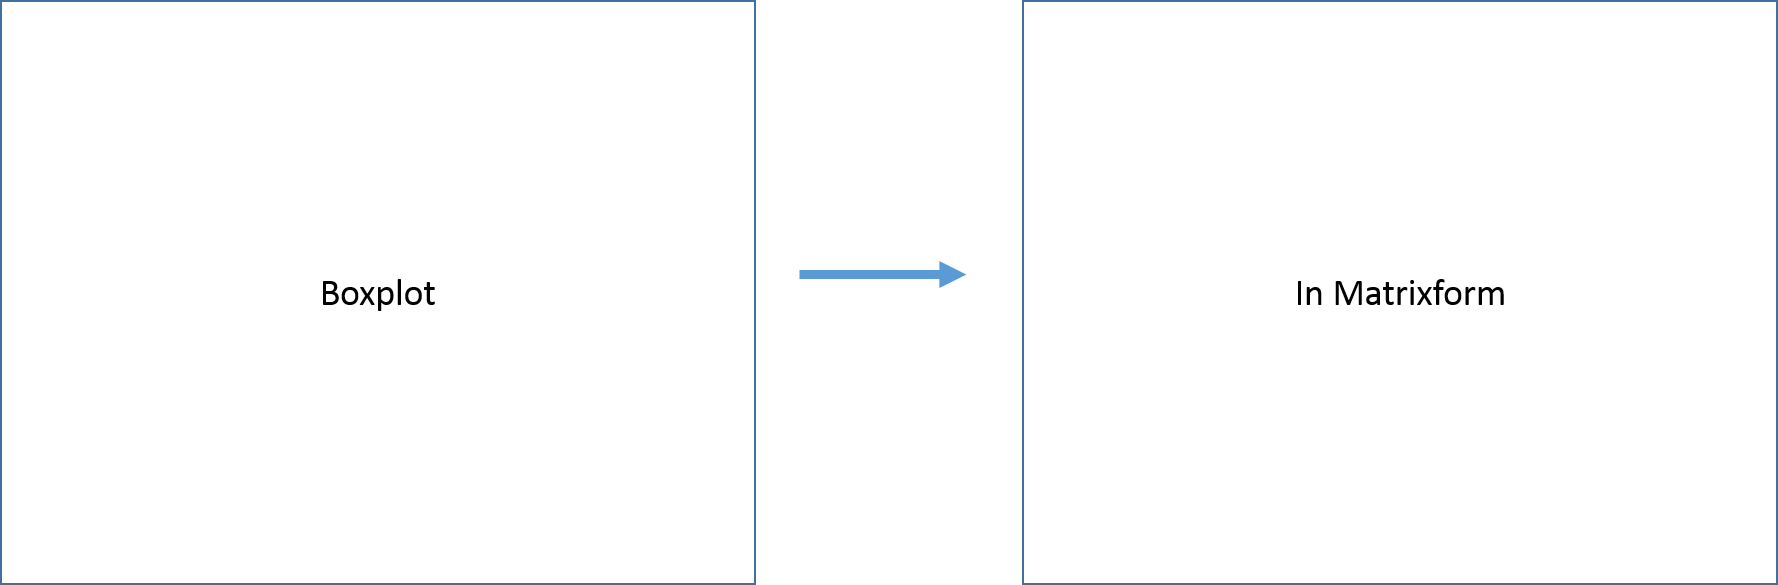
\includegraphics[scale=0.5]{testbild}
		\caption{Umformung des Boxplots in Matrixform}
	\end{figure}
	\\
	Da diese Matrizen je nach Parameter ziemlich groß werden können, sollen sie approximiert werden. Nach der Darstellung eines Beispiels werden im nächsten 
	Kapitel diverse Approximationsmethoden vorgestellt.
	\subsection{Beispiel: das invertierte Pendel}
	Als Beispiel dient das Modell des invertierten Pendels auf einem Wagen. Bei diesem Modell wird ein starres 
	invertiertes Pendel rotationsfähig auf einem Wagen montiert. Beide Körper, Pendelmasse und Wagen, werden als 
	konzentrierte Punktmassen angenommen. Zur Balancierung des Pendels können Kräfte $u$ auf den Wagen angewandt 
	werden um ihn in der Horizontalen zu stabilisieren. Die Dynamik des Wagens wird in diesem Modell vernachlässigt, 
	stattdessen konzentriert man sich auf den Auslenkungswinkel $\varphi$ des Pendels von der Vertikalen und auf die 
	Winkelgeschwindigkeit $\dot{\varphi}$ im Zustandsraum $(\varphi,\dot{\varphi})\in \mathds{R}^2$. \\
	Das Pendel befindet sich im höchsten Punkt in einer instabilen Ruhelage. Verlässt es diese Ruhelage um einen 
	Winkel $\varphi$, so muss dem Pendel wieder Energie hinzugefügt werden um es wieder in den Zustand der instabilen 
	Ruhelage zurück zu versetzen. Das mathematische System zu dieser Zustandsrückführung definiert sich 
	wiefolgt (vgl. \citep{Grune2005}):
	\begin{eqnarray}
		\dot{x_1} &=& x_2 \\
		\dot{x_2} &=& \frac{\frac{g}{l}\sin (x_1)-\frac{1}{2}m_rx_2^2\sin (2x_1)-\frac{m_r}{ml}\cos (x_1)u}{\frac{4}{3}-m_r\cos ^2(x_1)}
	\end{eqnarray}
	wobei $x_1=\varphi$, $x_2=\dot{\varphi}$, $m_r=\frac{m}{m+M}$ das Massenverhältniss zwischen Pendelmasse und 
	Wagenmasse, $m=2kg$, $M=8kg$, $l=0.5m$ Länge des Pendels und $g=9.8\frac{m}{s^2}$ die Gravitationskonstante. \\
	Die schrittweisen Stabilisierungskosten des inversen Pendels ergeben sich aus
	\begin{equation}
		q(x,u)=\frac{1}{2}(0.1x_1^2+0.05x_2^2+0.01u^2).
	\end{equation}
	Berechnet man auf Basis dieses mathematischen Modells nun die Wertefunktion $V_\mathcal{P}$ wie in 
	\ref{sec:valuef} definiert, so ergibt sich folgendes Bild:
	\begin{figure}[h]
		
		\center
		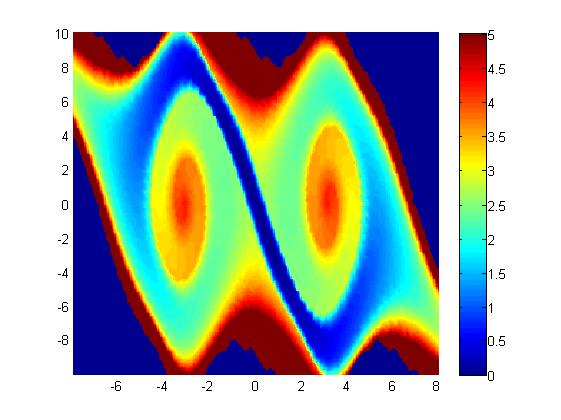
\includegraphics[scale=0.55]{valuefunction_plot_256.jpg}
		\caption{\label{pic:Vapp}Approximierte Wertefunktion $V_\mathcal{P}$ bei Simulationstiefe 16}
	\end{figure}
	\newline
	Ausgehend von der Ruhelage des Pendels im Punkt $(0,0)$ im Phasendiagramm nehmen die Kosten zur Stabilisierung 
	des Pendelsystems zu.
	\textcolor{red}{hier noch etwas aus dem gaio paper eintragen}
	\newpage
\section{Niedring-Rang-Approximation einer Matrix}
	Je nach Tiefe der Simulation bzw. der Dimension des zugrunde liegenden Raumes (vgl. \textbf{Fluch der Dimension} 
	nach Bellman \citep{Bellman1961}) können gigantische Matrizen entstehen. Da die gängigen Rechner bei der 
	Speicherung solcher Matrizen schnell an ihre Grenzen stoßen, soll nun für die Wertematrix $V$ eine Niedrig-Rang-
	Approximation der Form
	\begin{equation}
		\label{eq:approx}
		V(x)\approx \sum_{i=1}^k\sigma_i u_i(x) v_i^T(x)
	\end{equation}
	gefunden werden, wobei $\sigma_i\in \mathds{R}$ Konstanten und $u_i, v_i$ Vektoren im $\mathds{R}^n$ sind. Im Folgenden werden einige Näherungen vorgestellt.
	\subsection{Singulärwertzerlegung (SVD)}
		\label{sec:SVD}
		\subsubsection{Definition}
		Die klassische Singulärwertzerlegung ist eine Erweiterung der Diagonalisierung von reellen quadratischen 
		Matrizen auf komplexe $\mathds{R}^{m\times n}$-Matrizen und gerade in der numerischen Mathematik von großem 
		Nutzen. Sie ist folgendermaßen definiert.		
		\begin{Definition}
		Sei A eine komplexe $m\times n$-Matrix von Rang $r$. Die Singulärwertzerlegung von A ist gegeben durch (vgl. 			\cite{deuflhard2008})
		\begin{equation*}
			\label{eq:SVD}
			A=U\Sigma V^* 
		\end{equation*}
		wobei
		\begin{itemize}
			\item $U$ eine unitäre $m\times m$-Matrix ist,
			\item $V^*$ die Adjungierte einer $n\times n$-Matrix $V$ ist und
			\item $\Sigma$ eine reelle $m\times n$-Diagonalmatrix der Form \[
	 		\Sigma = \left(\begin{array}{ccc|ccc}
					\sigma_1 &          &         &       & \vdots &       \\
         			& \ddots   &         & \cdots & 0      & \cdots \\
         			&      &\sigma_r &        & \vdots &        \\
					\hline
        			 &  \vdots  &        &       & \vdots &        \\
					\cdots   & 0       & \cdots   & \cdots & 0      & \cdots \\
        			 &  \vdots  &         &        & \vdots &        \\
					\end{array}\right)
			\]
			Die Einträge $\sigma_i>0$, $i=1...r$, $\sigma_1>...>\sigma_r$ heißen Singulärwerte von A. Die Spalten von $U$, $u_i$, heißen linke Singulärvektoren, die Spalten von $V$, $v_i$, heißen rechte Singulärvektoren.
		\end{itemize}
		\end{Definition}
		\begin{Bemerkung}
			$A$ kann auch geschrieben werden als die Summe von Rang-1-Matrizen:
			\begin{equation*}
				\label{eq:SVDsum}
				A=\sum_{i=1}^r\sigma_i u_i v_i^T
			\end{equation*}
			Die $\sigma_i$ sind dabei die Singulärwerte von $A$ und $u_i$ und $v_i$ die Zeilen von $U$ bzw. $V$.
		\end{Bemerkung}
		Die Berechnungskosten, die für das Ausführen der Matrixzerlegung benötigt werden, betragen $\mathcal{O}(min(mn^2,m^2n))$ (vgl. \cite{mahoney2008}).
	%	\newline 
		\subsubsection{Fehlerapproximation}
		Im Folgenden wollen wir die Wertematrix $V$ so approximieren, dass der Fehler 
		\begin{equation*}
			e(D)=||V-D||_\xi
		\end{equation*}
		bezüglich einer Norm $\xi$ möglichst klein wird für Matrizen $D$ von Rang $rank(D)\leq k$. $\xi=2$ bezeichnet hierbei die 2-Norm ($||A||_2=\left(\sum_{i,j}|a_{ij}|^2\right)^\frac{1}{2}$), $\xi=max$ bezeichnet die Maximumsnorm ($||A||_{max}=\max_{i,j}|a_{ij}|$) und $\xi=F$ verwendet die Frobeniusnorm ($||A||_F=(\sigma_1^2+...+\sigma_r)^\frac{1}{2}$).
		\newline

		Die erste Frage, die es dabei zu klären gilt, ist die nach der Existenz einer  "besten" Rang-k-Approximation.
		\begin{Satz}{(Eckart-Young)}
			Sei eine Matrix $V$ von Rang $r$ gegeben durch \ref{eq:SVD} und $k<r$. Die beste Rang-$k$-Approximation 
			von $V$, also eine Matrix, die
			\begin{equation*}
				\min_{rank(B)\leq k}||V-B||_2	
			\end{equation*}		
			erfüllt, ist gegeben durch
			\begin{equation*}
				 V_k=\sum_{i=1}^k\sigma_i u_i v_i^T
			\end{equation*}
			und 
			\begin{equation*}
				||V-V_k||_2=\sigma_{k+1}
			\end{equation*}
			wobei $\sigma_{k+1}$ der (k+1)-te Singulärwert von $V$ ist. Dies impliziert, dass für Singulärwertzerlegungen von Rang $k\geq r$ gilt: $||V-V_k||_2=0$.
		\end{Satz}
		\begin{Beweis}
			Für einen Beweis siehe \cite{Golub2013}.
		\end{Beweis}
		Zusammenfassend kann über die Matrixzerlegung mithilfe der Singulärwertzerlegung folgendes gesagt werden: \newline
		\newline
		\textbf{Vorteil:}
		\begin{itemize}
			\item Die Singulärwertzerlegung ist die bezüglich der Maximumsnorm "beste" \ Rang-k-Approximation einer Matrix.
\end{itemize}		
		\textbf{Nachteile:} 
		\begin{itemize}
			\item Sehr hohe Kosten zum Ausführen der Singulärwertzerlegung. Die Kosten der Rang-k-Singulärwertzerlegung betragen $\mathcal{O}(kmn)$ (siehe \citep{Drineas2006}).
			\item Zur Approximation werden keine Einträge der Zielmatrix verwendet.
		\end{itemize}
		Im nächsten Abschnitt werden zwei Verfahren vorgestellt, welche zur Approximation Spalten und Zeilen der 
		Eingabematrix verwenden.
	\subsection{CUR-Zerlegung}	
		\label{subsec:CUR}
		\subsubsection{Definition}
		Bei der CUR-Zerlegung werden im Gegensatz zur CX-Zerlegung Spalten und Zeilen der zu approximierenden Matrix 
		verwendet. Die Matrix C enthält dabei Spalten von $V$ und Zeilen werden in R gefasst. Die Matrix $U$ wird 
		dann so gewählt, dass der Fehler zwischen $V$ und $\tilde{V}=CUR$ bezüglich einer Norm (i.d.R der Frobenius- oder Spektralnorm) minimal wird. \\
		Die Struktur der CUR-Zerlegung stellt sich wiefolgt dar:
		\[
			\underbrace{\left(\begin{array}{ccccc}
					  &   &  & & \\ & &  & &  \\ & & V &  &   \\ & & &  &   \\ & & &  &   \\ 
					\end{array}\right)}_{m\times n}
			\approx 
			\underbrace{\left(\begin{array}{ccc}
					 &   &   \\  &   &   \\ & C &   \\ &   &   \\ &   &   \\
					\end{array}\right)}_{m\times c}\cdot 
			\underbrace{\left(\begin{array}{ccc}
					  &   &   \\ & U &   \\ &   &   \\ 
					\end{array}\right)}_{c\times r}\cdot  
			\underbrace{\left(\begin{array}{ccccc}
					  &   &  & & \\ & & R & &  \\ & & &  &   \\ 
					\end{array}\right)}_{r\times n}			
		\]
		Da wir nun die Idee hinter der CUR-Zerlegung sowie deren Struktur festgelegt haben, können wir die 
		Approximation mathematisch definieren.
		\begin{Definition}{(vgl. \citep{Drineas2009})}
			Gegeben sei eine Matrix $V\in \mathds{R}^{m\times n}$. Sei $C\in\mathds{R}^{m\times 
			c}$ eine Matrix, welche aus $c$ Spalten von $V$ besteht, und $R\in\mathds{R}^{r\times n}$ eine Matrix, 
			deren $r$ Zeilen aus Zeilen von $V$ bestehen. Dann ist die Matrix $V'=CUR$ für jede beliebige Matrix $U
			\in\mathds{R}^{c\times r}$ eine Spalten-Zeilen-basierte Approximation von $V$, beziehungsweise eine $CUR
			$-Zerlegung von $V$.
		\end{Definition}
		Besonders kritisch bei der Berechnung der Zerlegung ist, welche Zeilen bzw. Spalten für die Approximation 
		verwendet werden. Dafür werden im Folgenden zwei verschiedene Verfahren und die resultierenden 
		Approximationen dargestellt.
		\subsubsection{Zufällige Spaltenselektion auf Basis der Gleichverteilung}
		Der erste intuitive Ansatz zur Selektion von Matrixindizes ist der, der auf der \textbf{Gleichverteilung} 
		der Indexwahrscheinlichkeiten beruht. Das heißt, die Wahrscheinlichkeit, dass eine beliebige Zeile oder 
		Spalte einer Matrix ausgewählt wird, ist für alle relevanten Matrixbestandteile identisch. \newline Im Falle einer $m
		\times n$-Matrix ergibt sich explizit $\sigma_i=\frac{1}{m}$ für die Wahrscheinlichkeit zur Selektion der 
		$i-$ten Zeile respektive $\sigma_j=\frac{1}{n}$ für die der $j-$ten Spalte. Man sieht sehr schön, dass die Selektions-Wahrscheinlichkeit einer Zeile oder Spalte unabhängig von dem ausgewählten Index ist.\newline
		\newline
		\begin{table}[h]
		\center
		\fbox{
		\begin{minipage}{16cm}
		\vspace{5mm}
			\textbf{CUR-Zerlegung bei Gleichverteilung} \newline
			\newline
			\begin{tabular}{ll}
				\textbf{Input:} & Matrix $V\in\mathds{R}^{m\times n}$, Reihenanzahl $r\leq m$, Spaltenanzahl $c\leq n$\\
				(i) & für $t=1\dots r$ wähle die $i-$te Zeile mit Wahrscheinlichkeit $\sigma_i=\frac{1}{m}$ und \\
				 & füge sie als Zeile $t$ der Matrix $R$ hinzu. Wurde diese Zeile bereits ausgewählt, \\
				 & wiederhole den Selektionsschritt. Erhalte so die Reihenmatrix $R$. \\
				(ii) & für $t=1\dots c$ wähle die $j-$te Spalte mit Wahrscheinlichkeit $\sigma_j=\frac{1}{n}$ und\\ & füge sie als Spalte $t$ der Matrix $C$ hinzu. Wurde diese Spalte bereits
				\\ &  ausgewählt, wiederhole den Selektionsschritt. Erhalte so die Zeilenmatrix $C$. \\
				(iii) & Definiere die Matrix $U$ als $U=C^+AR^+$, wobei $X^+$ die Moore-Penrose- \\ & Inverse 
				\citep{penrose1955}von X ist. \\
				\textbf{Output:} & Spaltenmatrix $C\in\mathds{R}^{m\times c}$, Zeilenmatrix $R\in\mathds{R}^{r\times n}$ und Matrix $U\in\mathds{R}^{c\times r}$ \\
			\end{tabular}
			\vspace{2mm}
		\end{minipage}
		}
		\newline
		\caption{Der Algorithmus \textit{randCUR} zur Bestimmung der CUR-Zerlegung auf Grundlage der gleichverteilten Wahrscheinlichkeiten für die Selektion von Spalten- bzw. Zeilen-Indizes}
		\end{table}
		\textbf{Vorteile:}
		\begin{itemize}
		\item Geringe Berechnungskosten $\mathcal{O}(l+r+m+n)$, da die Singulärwertzerlegung zur Indexauswahl nicht benötigt wird.
		\item Trotzdem relativ gute Approximationsergebnisse
		\end{itemize}
		\textbf{Nachteile:}
		\begin{itemize}
		\item Zufällige Selektion lässt keine Rückschlüsse auf den größtmöglichen Fehler zu.
		\item Langsamere Konvergenz (vgl. \ref{sec:gleichv}) im Vergleich zur Singulärwertzerlegung
		\end{itemize}
		\subsubsection{Spaltenselektion anhand des Leverage Scores}
		Im Folgenden wird das Verfahren der Spaltenselektion anhand eines statistischen Wertes (engl.: 
		\textit{leverage score}) nach Mahoney und Drineas \citep{mahoney2008} dargestellt. Dabei wird ein Rating erzeugt, welche den 
		Einfluss einer Spalte/Zeile auf die "beste" Rang-k-Approximation, also die Singulärwertzerlegung von Rank $k$, der Matrix beschreibt. Dieser spezifische Wert beschreibt, mit welcher Wahrscheinlichkeit eine Zeile/Spalte selektiert und zur Approximationsmatrix hinzugefügt wird. \newline
		\newline	
		\textbf{Bestimmung des statistischen Einflusswertes einer Spalte/Zeile:} \newline 
		Aus \ref{eq:SVDsum} wissen wir, dass sich die $j$-te Spalte einer Zielmatrix $V$ von Rang $r$ darstellen lassen kann als
		\begin{equation*}
			V^j=\sum_{\xi=1}^r(\sigma_\xi u^\xi )v_j^\xi
		\end{equation*}
		bzw. deren "beste" \ Rang-k-Approximation durch
		\begin{equation*}
			V^j=\sum_{\xi=1}^k(\sigma_\xi u^\xi )v_j^\xi
		\end{equation*}
		wobei $u^\xi$ der $\xi$-te linke Singulärvektor und $v_j^\xi$ die $j$-te Koordinate des $\xi$-ten rechten 
		Singulärvektors ist. Der \textbf{statistische Einflusswert} einer Spalte von $V$ kann nun gemessen werden durch
		\begin{equation}
			\label{eq:score}
			\pi_j=\frac{1}{k}\sum_{\xi=1}^k(v_j^\xi)^2 \hspace{2cm} j\in [1,n]
		\end{equation}
		Er gibt an, wie groß der Einfluss einer Spalte auf die durch die Singulärwertzerlegung definierte "beste" \ Rang-k-Approximation $V_k$ ist. \\
		Diese Einflusswerte bilden eine Wahrscheinlichkeitsverteilung auf den $n$ Spalten und es gilt: $\sum_{j=1}^n\pi_j=1$ und $\pi_j\geq 0$. \newline
		Das Selektieren der Spalten wird anschließend mithilfe des Algorithmus' COLUMNSELECT (vgl. \citep{mahoney2008}) durchgeführt: 
		\begin{enumerate}
			\item \textbf{Input:} Matrix $V\in \mathds{R}^{m\times n}$ und Fehlerparameter $\epsilon$
			\item Berechne die ersten $k$ rechten Singulärvektoren ($v_1,...,v_k$) von V und die statistischen Einflusswerte \ref{eq:score} der Spalten von V.
			\item Verwende die $j$-te Spalte von V mit Wahrscheinlichkeit $p_j=min\{1,c\pi_j\}$, wobei $c=\mathcal{O}(k \log \frac{k}{\epsilon^2})$
			\item \textbf{Output:} Matrix $C$, welche aus den selektierten Spalten von $A$ besteht.
		\end{enumerate}
		Mithilfe dieses Algorithmus' entsteht eine Matrix $C$, die $c'\leq c$ der selektierten Spalten verwendet. Die 
		Kosten zur Ausführung des Algorithmus' beruhen hauptsächlich auf der Berechnung der ersten $k$ 
		Singulärvektoren und sind daher $\mathcal{O}(mnk)$ \citep{mahoney2008}.\newline
		Zur Berechnung der Matrizen $C,U$ und $R$ wird abschließend folgender Algorithmus ALGORITHMCUR (vgl. \citep{mahoney2008}) verwendet: \newpage
		\begin{table}[h]
		\center
		\fbox{
		\begin{minipage}{16cm}
		\vspace{5mm}
			\textbf{ALGORITHMCUR} \newline
			\newline
			\begin{tabular}{ll}
				\textbf{Input:} & Matrix $V\in\mathds{R}^{m\times n}$, Zielrang $k$, Fehlerparameter $\epsilon$ \\
				(i) & Wende COLUMNSELECT auf $A$ an mit $c=\mathcal{O}(k \log \frac{k}{\epsilon^2})$ und berechne somit\\
				 &  die Matrix $C$ \\
				(ii) & Wende COLUMNSELECT auf $A^T$ an mit $r=\mathcal{O}(k \log \frac{k}{\epsilon^2})$ und berechne 
				  \\ &somit die Matrix $R$ \\
				(iii) & Definiere die Matrix $U$ als $U=C^+AR^+$, wobei $X^+$ die Moore-Penrose- \\ & Inverse 
				\citep{penrose1955}von X ist \\
				\textbf{Output:} & Spaltenmatrix $C$, Zeilenmatrix $R$ und Matrix $U$ \\
			\end{tabular}
			\vspace{2mm}
		\end{minipage}
		}
		\newline
		\caption{Der Algorithmus ALGORITHMCUR zur Bestimmung der CUR-Zerlegung mithilfe des \\ Leverage Scores}
		\end{table}
		Die Wahrscheinlichkeit für die Auswahl einer der $c$ Zeilen bzw. $r$ Reihen erfolgt dabei proportional zur Einflussrate der entsprechenden Matrixeinträge. \newline
		\newline
		Die mithilfe des Algorithmus' konstruierte approximative Matrix $V'=CUR$ erfüllt nun, dass
		\begin{equation*}
			||V-V'||_F\leq (2+\epsilon )||V-V_k||_F
		\end{equation*}		
		mit hoher Wahrscheinlichkeit (m.h.W.) (vgl. \citep{mahoney2008}). \newline
		\newline
		Die Rate $(2+\epsilon)$ kann mit einer Variation des Algorithmus' noch weiter verbessert werden \citep{Drineas2009}. Bei dieser Methode wird die Matrix $R$ abhängig von den für die Matrix $C$ gewählten Zeilen berechnet. Durch diese Abwandlung verringert sich der Fehler m.h.W. zu
		\begin{equation*}
			||V-CUR||_F\leq (1+\epsilon)||V-V_k||_F
		\end{equation*}
		Dies ist nur eine Möglichkeit eine approximative $CUR$-Zerlegung der Matrix $V$ zu finden. Weitere werden in 
		folgender Tabelle gezeigt: \newline
		\begin{figure}[h]
			\begin{tabular}{l||c|c|c|c}
		 		& Anzahl Spalten c & Anzahl Reihen r & rank(U) & $||V-CUR||_F^2\leq$ \\
		 		\hline \hline
		 		Drineas et al. 2003 \citep{drineas2003} & $\frac{k}{\epsilon^2}$ & $\frac{k}{\epsilon^2}$ & $k$ & $||V-V_k||_F^2+\epsilon||A||^2_F$ \\
		 		\hline
		 		Drineas et al. 2008 \citep{Drineas2009} & $\frac{k\log k}{\epsilon^2}$ & $\frac{k\log k}{\epsilon^4}$ & $\frac{k\log k}{\epsilon^2}$ & $(1+\epsilon)||V-V_k||^2_F$ \\
		 		\hline
		 		Wang et al. 2013 \citep{Wang2013}& $\frac{k}{\epsilon}$ & $\frac{k}{\epsilon^2}$ & $\frac{k}{\epsilon}$ & $(1+\epsilon)||V-V_k||^2_F$
			\end{tabular}
			\caption{Tabelle über verschiedene CUR-Approximationen}
		\end{figure}
		
		\textbf{Vorteile:}
		\begin{itemize}
			\item Zeilen und Spalten der ursprünglichen Matrix werden verwendet.
			\item Auch bei der Selektion von nur einer geringen Anzahl an Spalten/Zeilen ($\approx\frac{1}{10}$ aller Spalten) wird bereits annähernd ein voller Rang der Matrix $\tilde{V}$ erreicht.
		\end{itemize}
		\newpage
		\textbf{Nachteile:} 
		\begin{itemize}
			\item Die approximierende Matrix ist nicht mehr von der Form \ref{eq:approx}
			\item Die Hauptkosten dieses Verfahrens zur Auswahl der Spalten bzw. Zeilen resultieren aus der Berechnung der relativ teuren Singulärwertzerlegung $\rightarrow$ hohe Berechnungskosten
		\end{itemize}
		\newpage
\section{Berechnung der Residuen}
\subsection{Definition}
	Für die exakte Wertefunktion $V$ gilt nach Bellmann, dass
	\begin{eqnarray*}
		V(x_k)&=&\inf_{u\in U^{\mathds{N}}}\{q(x_k,u)+V(f(x_k,u))\} \\
			&=&q(x_k,u_k^*)+V(f(x_k,u_k^*))
	\end{eqnarray*}
	mit dem minimierenden $u_k^*$, falls das Optimum angenommen wird, wobei $V(f(x_k,u))=:V(x_{k+1})$. Da $q(x,u)>0 \hspace{1mm}$ für $x\neq 0$ gilt also insbesondere, dass $V(x_k)>V(x_{k+1})$. \newline
	\newline
	Mit dieser Eigenschaft wird die Wertefunktion zu einer \textbf{Lyapunov-Funktion} (siehe \citep{Wiggins1990}), da gilt:
	\begin{enumerate}
		\item $V(x)\geq 0$ 
		\item $V(x)=0 \Leftrightarrow x=0$
		\item $V(x_k)>V(x_{k+1})$
	\end{enumerate}
	Leider ergibt sich bei der approximierenden $CUR$-Zerlegung $\tilde{V}$ das Problem, dass die Bedingung (iii) nicht 
	mehr notwendigerweise erfüllt ist. \\
	Für den resultieren Fehler berechnet man dazu das \textbf{Residuum} der Bellman-Gleichung. Dieses ist gegeben 
	durch
	\begin{equation}
		\label{eq:residuum}
		R(x)=\tilde{V}(x)-\inf_{u}\{q(x,u)+\tilde{V}(f(x,u))\}.
	\end{equation}
	mit
	\begin{equation}
		\tilde{u}(x)=argmin_{u\in U^{\mathds{N}}}\{q(x,u)+\tilde{V}(f(x,u)\}
	\end{equation}
	Im Falle des Erfüllens der Bedingung (iii) ergibt sich
	\begin{equation}
		R(x)\geq 0 \hspace{1cm}\forall x\in X
	\end{equation}
	da $q(x,u)\geq0$ für alle $x\in X$. \\
	Typischerweise ist diese Bedingung aber nicht für alle $x\in X$ erfüllt. Als alternative Formulierung soll 
	deshalb die Menge $\bar{S}=\{x\in X| R(x)<0\}$ bezüglich des Lebesque-Maßes möglichst geringes Volumen besitzen.
	\subsection{Beispiel: Residuum der exakten Wertefunktion}
	Die Berechnung des Residuums soll anhand der exakten Wertefunktion verdeutlicht werden. Diese exakte Wertematrix 
	relativ zur Partition $\mathcal{P}$ entsteht, wie in \ref{eq:bellman} beschrieben, durch Anwendung des 
	Optimalitätsprinzipes nach Bellman. Vergleicht man dieses nun mit der Definition des Residuums (siehe \ref{eq:residuum}), so liegt der Rückschluss nahe, dass das Residuum für die Wertefunktion trivial für alle Werte von $x$ ist (also $R(x)=0 \hspace{2mm}\forall x$). Wie Abbildung \ref{pic:res_exakt} aber verdeutlicht, gilt dies nicht 
	für die gesamte Wertefunktion, sondern nur für den stabilisierbaren Bereich. Der Grund dafür liegt in der 
	Konstruktion von $V$ nach dem Optimalitätsprinzip:
	\begin{equation*}
		V(x)=\inf_{u}\{q(x,u)+V(f(x,u))\}
	\end{equation*}
	Sei $x\in X\setminus S$ nun nicht stabilisierbar und $f(x,u)$ weiterhin Element in $X\setminus S$. Auch wenn 
	\begin{figure}[h]
	\center
		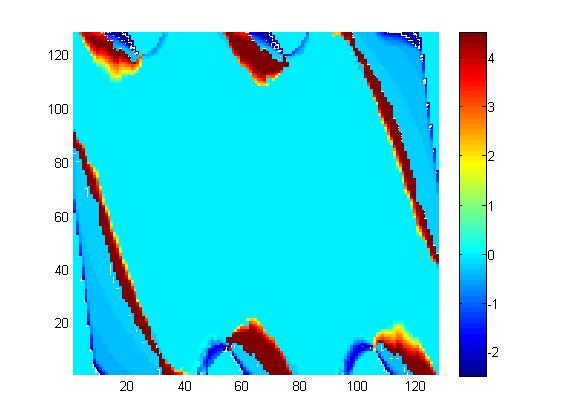
\includegraphics[scale=0.4]{Residuum_exactV_depth14.jpg}
		\caption{\label{pic:res_exakt}Residuum der exakten Wertefunktion bei Simulationstiefe 14}
	\end{figure}
	$V(f(x,u))=-1$ nach Definition wegen der nicht vorhandenen Stabilisierbarkeit, so ist aber $q(x,u)$ definiert und nicht-negativ. Aus diesem Grund ergeben sich 
	am Rand und im nichtstabilisierbaren Bereich von $X$ Abweichungen beim Residuum. Da in der Anwendung aber 
	hauptsächlich der stabilisierbare Bereich von Relevanz ist, nehmen wir dieses Phänomen zur Kenntnis, ignorieren 
	es aber in den folgenden Experimenten und konzentrieren uns auf den stabilisierbaren Bereich $S$.
	\newpage
\section{Qualitativer Vergleich der Approximationsmethoden}
Im Folgenden werden einige Experimente zu den verschiedenen Methoden zur Rekonstruktion der Zielmatrix durchgeführt. Als Vergleichsobjekt dient dabei die Matrix der nötigen Kosten zur Stabilisierung eines inversen Pendels. Die Ergebnisse wurden mithilfe des graphentheoretischen Ansatzes von Grüne und Junge \citep{Grune2005} in Matlab\footnote{Verwendet wurde das Software-Paket GAIO$^\copyright$	 - Global Analysis of Invariant Objects für Matlab} bei Simulationstiefe 14 - entspricht einer resultierenden Kostenmatrix $V\in\mathds{R}^{128\times 128}$ - erstellt. Die Verfahren werden in Hinblick auf Konvergenzgeschwindigkeit, Akkuratesse und Standort der größten Fehler verglichen.
\subsection{Anwendung der Rang-k-Singulärwertzerlegung}
In Kapitel \ref{sec:SVD} wurde bereits festgestellt, dass die Singulärwertzerlegung die beste Rang-$k$-Annäherung einer Matrix $V$ bezüglich der Frobenius- bzw. Spektralnorm liefert. Leider beinhaltet dieses Faktum keine a-priori-Informationen, wie sich die Fehler in einem bestimmten Bereich der Matrix verhalten. \\
Aus diesem Grund werden folgend einige experimentelle Beobachtungen geliefert, die Rückschlüsse auf diese fehlenden Informationen geben sollen. 
\subsubsection*{Akkuratesse und Konvergenz}
\begin{figure}[h]
	
	\centering
	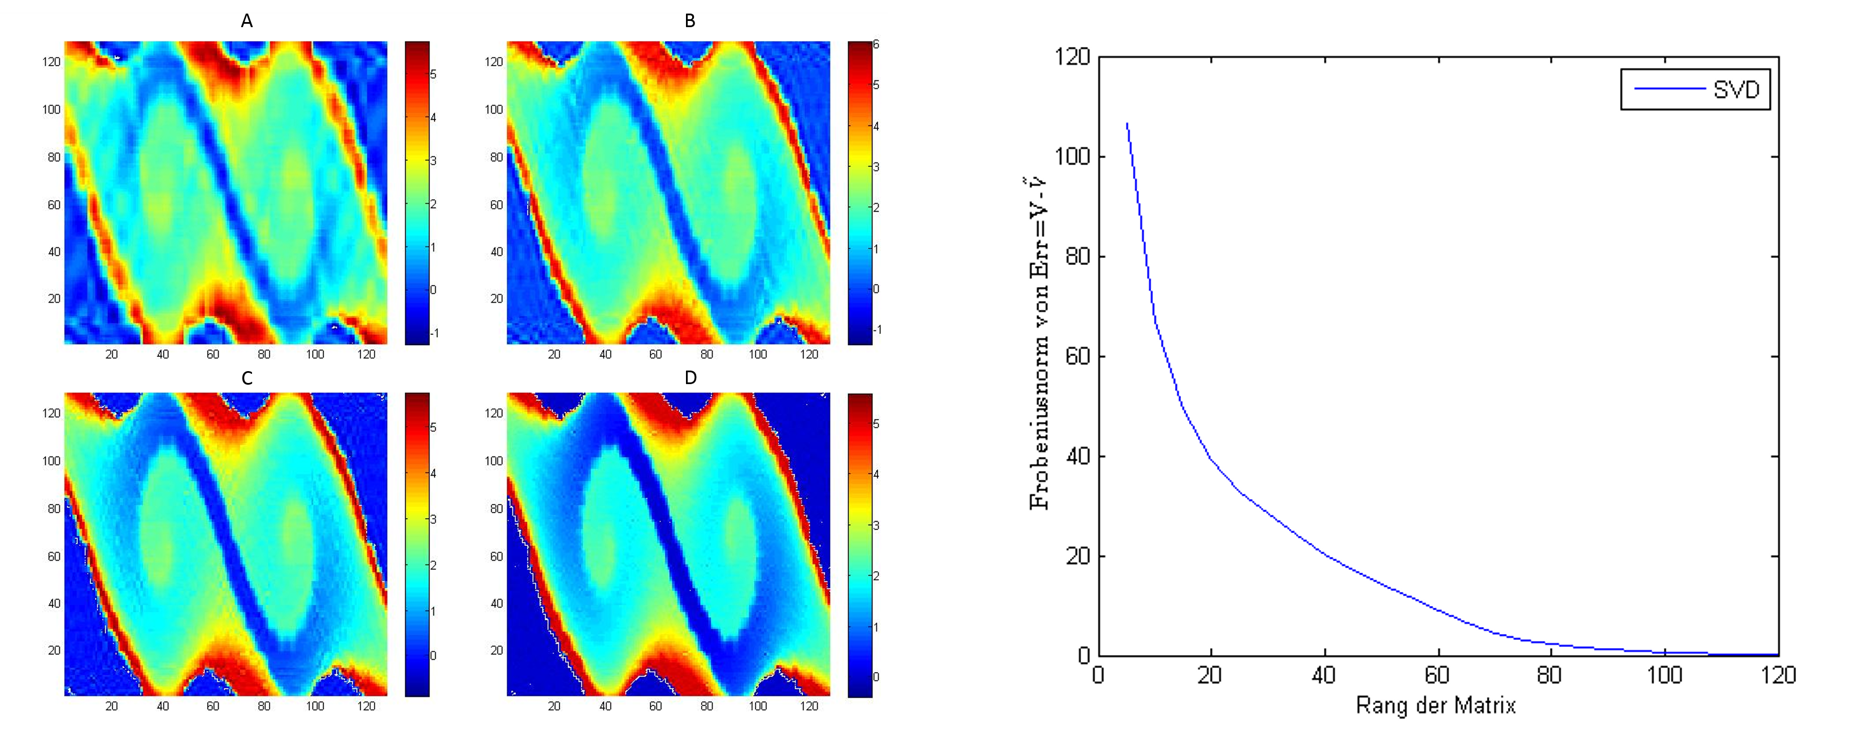
\includegraphics[scale=0.45]{SVD_plots_graph}
	\caption{\label{pic:SVD_plots}links: Boxplots der resultieren Approximationsmatrizen bei Auswahl der 10 (A), 20 (B), 30 (C) und 60 (D) oberen Singulärvektoren. rechts: resultierender Fehler der Rang-k-Singulärwertzerlegung bezüglich der Frobeniusnorm}
\end{figure}
Wie in der oberen linken Abbildung ersichtlich, ist schon bei der Auswahl der 20 - also ca. $\frac{1}{6}$ aller - oberen Singulärwerten klar die Struktur der ursprünglichen Matrix zu erkennen. Werden weitere Singulärwerte hinzugefügt, so verbessert sich das Bild zwar noch stetig, allerdings nur noch in geringerem Maße. Zieht man die 60 größten Singulärwerte in Betracht, also in etwa die Hälfte, so unterscheidet sich das Ergebnis kaum mehr von der Originalmatrix (vgl. Abbildung \ref{pic:Vapp}). \newline
\newline
Verdeutlicht wird dies auch durch den Plot des resultierenden Fehlers bezüglich der Frobeniusnorm (siehe Abbildung \ref{pic:SVD_plots} rechts). Die mit Hilfe der Singulärwertzerlegung erhaltene Approximationsmatrix konvergiert exponentiell in der Anzahl an gewählten Singulärwerten bzw. im Rang k der Approximation gegen die Zielmatrix $V$.
%\newpage
\subsubsection*{Fehlerlokalisierung}
Auch wenn wir nun wissen, dass der Fehler relativ schnell gegen Null konvergiert, so beinhaltet dies keine Informationen darüber, wo sich bei einer Rang-k-Approximation die größten Fehler befinden. In dem vorliegenden Fall sind wir vor allem an einer gewissen Genauigkeit innerhalb des stabilisierbaren Bereiches interessiert. Größere Fehler außerhalb dieses Bereiches können deshalb gegebenenfalls ignoriert werden.
\begin{figure}[h]
\center
	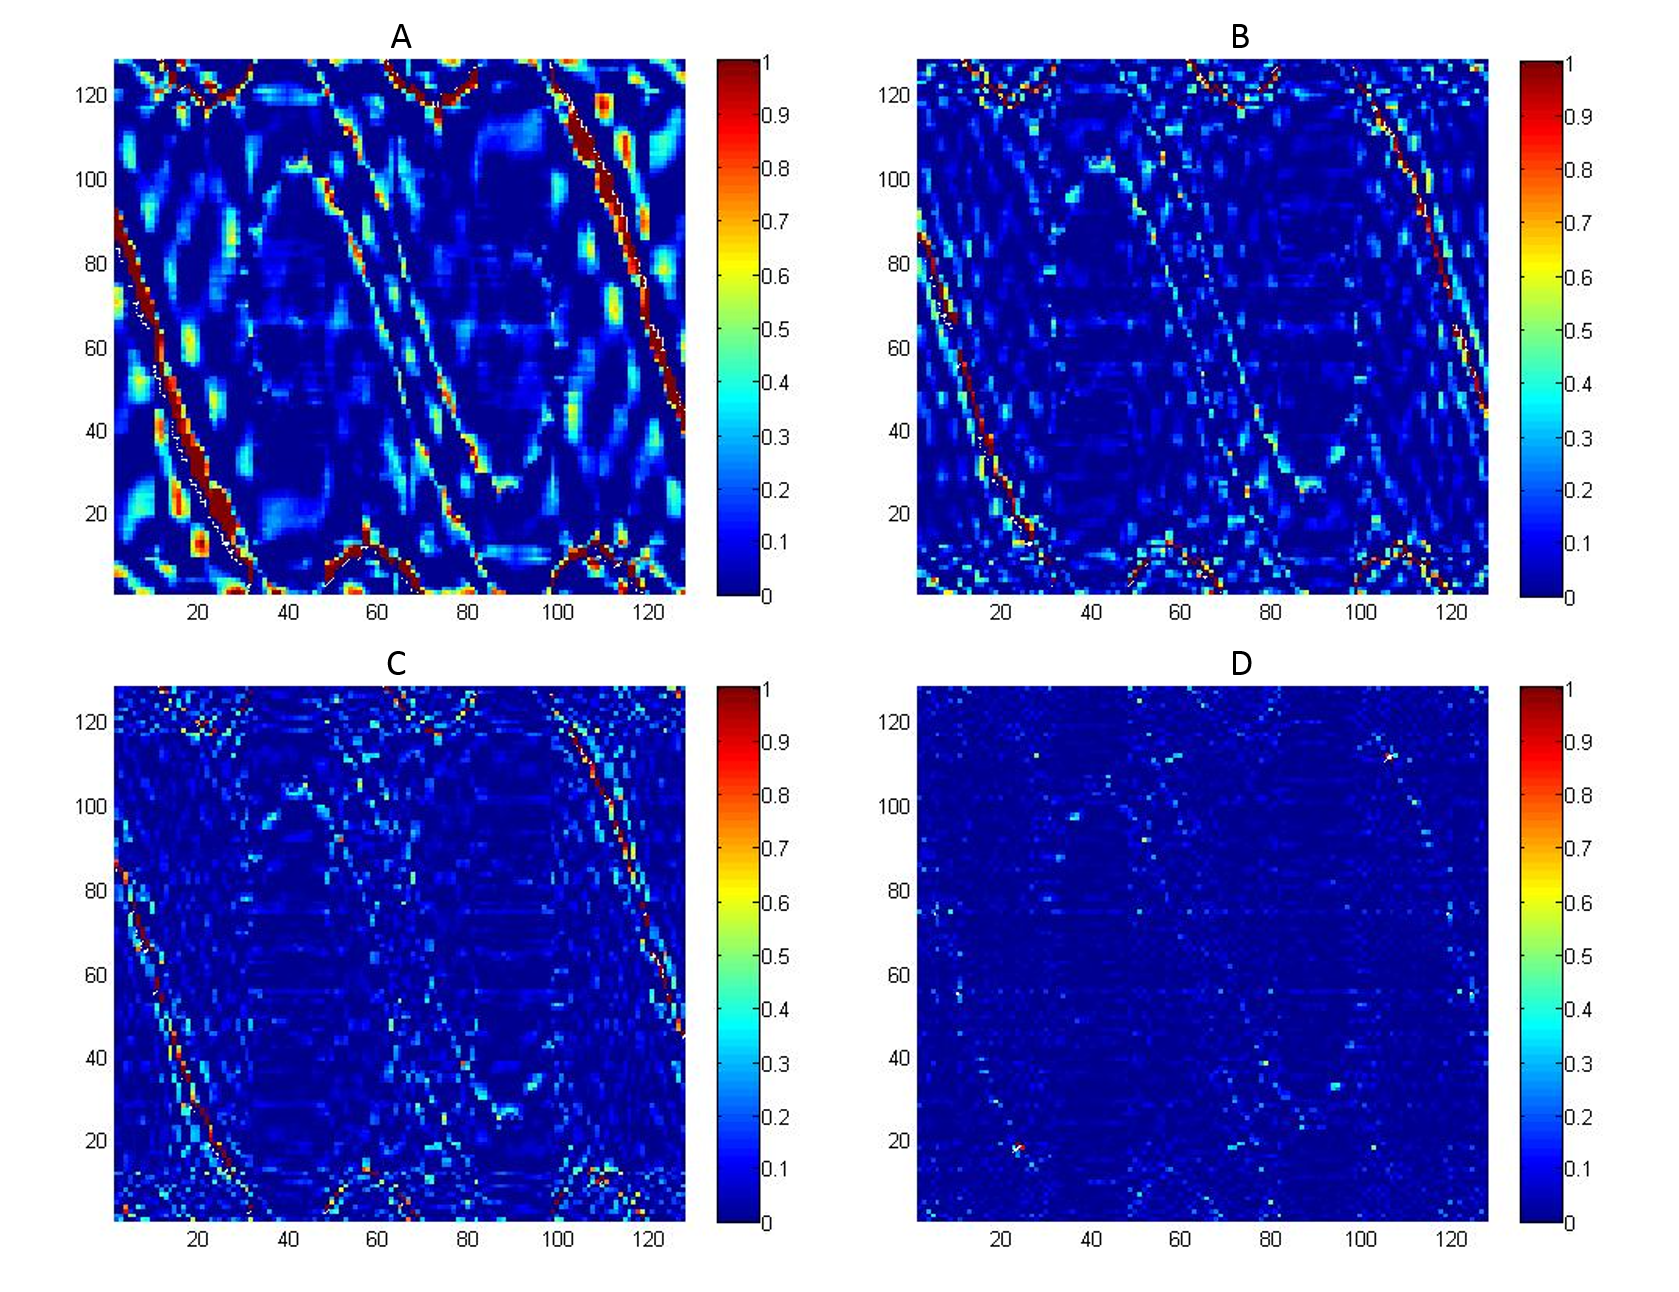
\includegraphics[scale=0.33]{SVD_errorloc.png}
	\caption{\label{pic:svd_errorloc}Lokalisierung der größten Fehler bei der Approximation durch die Singulärwertzerlegung von Rang 10 (A), 20 (B), 40 (C) und 60 (D)}
\end{figure}
Wie in Abbildung \ref{pic:svd_errorloc} zu sehen ist, befinden sich die größten Abweichungen der Approximation verglichen mit dem Original größtenteils am Rand des stabilisierbaren Bereiches. Während es bei der Singulärwertzerlegung von Rang 10 noch vereinzelt zu Abweichungen im Inneren kommt, stimmen die SVD von Rang 20 und höher im stabilisierbaren Bereich fast komplett überein und unterscheiden sich nur noch in der Größe der Abweichung am Rand des stabilisierbaren Bereiches.
\newpage
\subsubsection*{Residuum}
Für die positive Bewertung eines Verfahrens bezüglich des Residuums ist ausschlaggebend, wie viele Einträge der Residuenmatrix $R$ nicht-negativ sind. Wird diese Matrix als flache Oberfläche graphisch dargestellt, so lässt sich anhand der Farben der Wert der Matrixeinträge erkennen. Bei der SVD von Rang 10 und Rang 20 sind noch sehr deutlich rote und gelbe "Flecken" \ sichtbar, welche in der Graphik die Stellen mit negativem Residuum symbolisieren. Erst bei  Einbeziehung von mindestens 40 oberen Singulärwerten treten diese Punkte nur noch vereinzelt und mit kleinerem Volumen auf.
\begin{figure}[h]
	\center
	\includegraphics[scale=0.4]{svd_residuen}
	\caption{Darstellung der Residuen bei Anwendung der Singulärwertzerlegung von Rang 10 (A), 20 (B), 40 (C) und 60 (D). Zur besseren Übersicht wird das Ergebnis auf den Bereich $[-1,1]$ eingeschränkt.}
\end{figure}
\subsubsection*{Zusammenfassung}
\begin{itemize}
	\item[$+$] schnelle Konvergenz
	\item[$+$] innere Struktur der Matrix bleibt auch bei geringem Approximations-Rang erhalten
	\item[$+$] auch bei geringem Rang befinden sich die Fehler größtenteils am Rand des stabilisierbaren Bereiches
	\item[$+$] geringes Volumen des negativen Residuums
	\item[$-$] vergleichsweise sehr hohe Berechnungskosten
\end{itemize}
\newpage
\subsection{Anwendung der CUR-Zerlegung auf Basis der Gleichverteilung}
\label{sec:gleichv}
\begin{comment}
\subsubsection*{Akkuratesse und Konvergenz}
\begin{figure}[h]
\center
	\includegraphics[scale=0.3]{randCUR_plots2.png}
	\caption{Matrixplot der resultierenden Approximationen bei Auswahl von 10 (A), 20 (B), 40 (C), 60 (D) und 90 (E) Zeilen und Spalten}
\end{figure}

\subsubsection*{Fehlerlokalisierung}
\begin{figure}[h]
\center
	\includegraphics[scale=0.4]{randCUR_errorloc.png}
	\caption{SVD error}
\end{figure}
\subsection{Anwendung der CUR-Zerlegung auf Basis des Leverage Scores}
	Die numerische Berechnung der approximativen Matrix $C'=CUR$ wird in $R$\footnote{R Version 3.1.1, Script ausgeführt mithilfe RStudio Version 0.98.1017} durchgeführt. Dafür wird ein auf Drineas und Mahoney \citep{mahoney2008} basierender Algorithmus \citep{bodor2012} verwendet. \newline
	Die ursprünglich von Drineas et al. \citep{mahoney2008} veröffentlichte Methode verwendet eine Auswahl an Zeilen 
	und Spalten der Zielmatrix entsprechend der stochastischen Einflussrate. Dies impliziert einige numerische 
	Probleme, da die resultierenden Fehler zwischen Zielmatrix und $CUR$-Zerlegung je nach ausgewählten Zeilen/
	Spalten sehr stark variieren. Aus diesem Grund wurden Berechnungen mit unterschiedlichen Variationen dieser 
	Methode durchgeführt. \newline
	Die besten Ergebnisse wurden mit der Methode \textit{ortho.top.scores} erreicht. Bei dieser Variation des Algorithmus' werden die Spalten und Zeilen aufgrund der Linearkombination aus Einflusswert und "maximaler Orthogonalität" der Spalten bzw. Zeilen zueinander ausgewählt. \\
\subsection{Beispiel: das invertierte Pendel}
	\begin{figure}[h]
		\center
		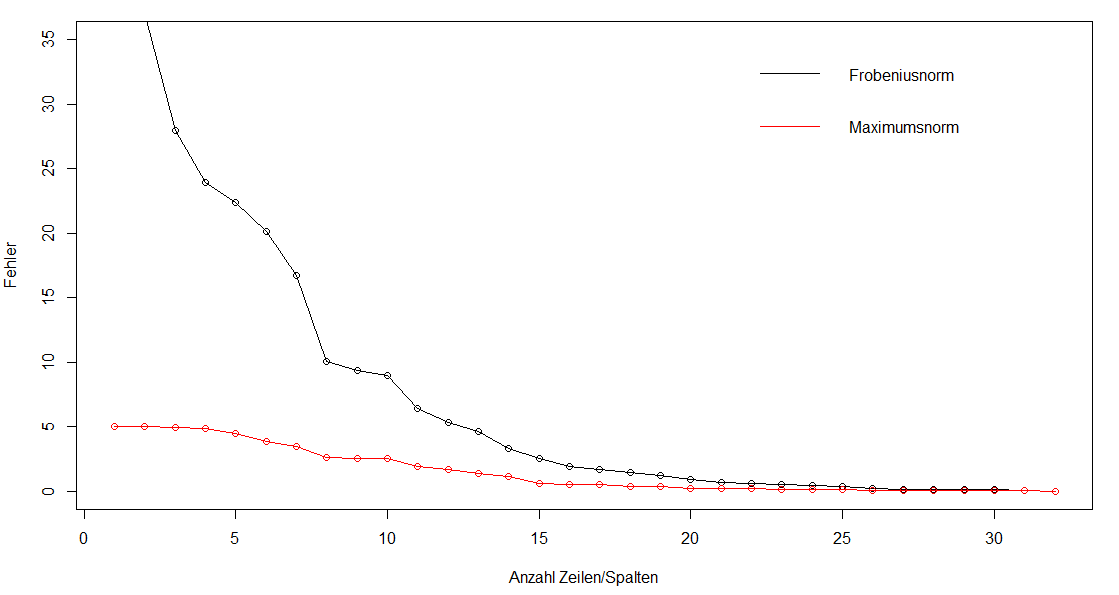
\includegraphics[scale=0.45]{Rplot_depth10.PNG}
		\caption{Plot der resultierenden Fehler bei einer 32x32-Matrix (schwarz) Frobeniusnorm (rot) Maximumsnorm}
	\end{figure}	
	\begin{figure}[h]
		\center
		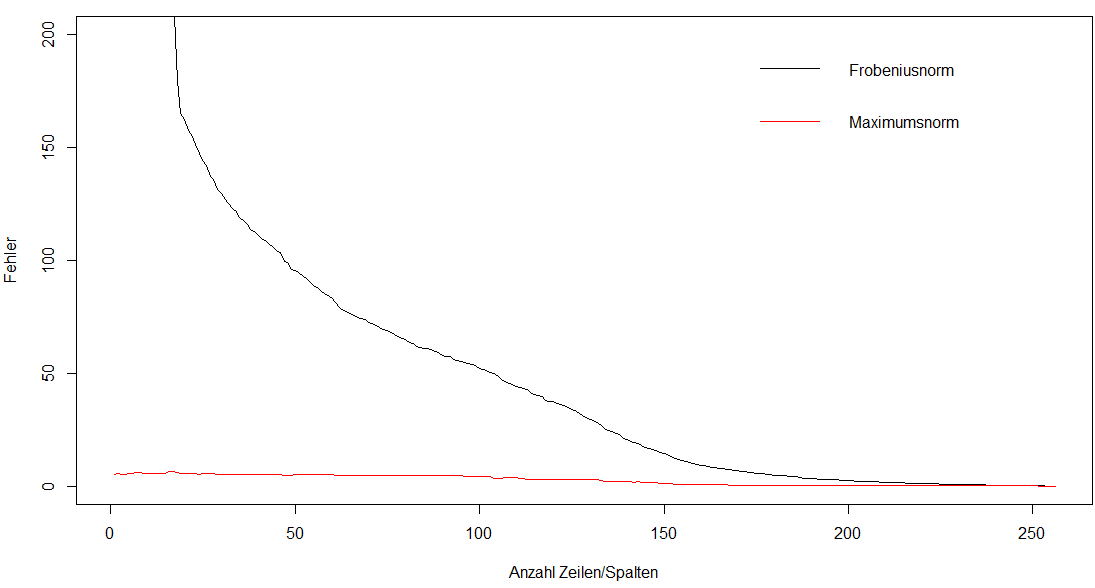
\includegraphics[scale=0.4]{Rplot_depth16_2.PNG}
		\caption{Plot der resultierenden Fehler bei einer 256x256-Matrix (schwarz) Frobeniusnorm (rot) Maximumsnorm}
	\end{figure}	
	\begin{figure}[h]
		\center
		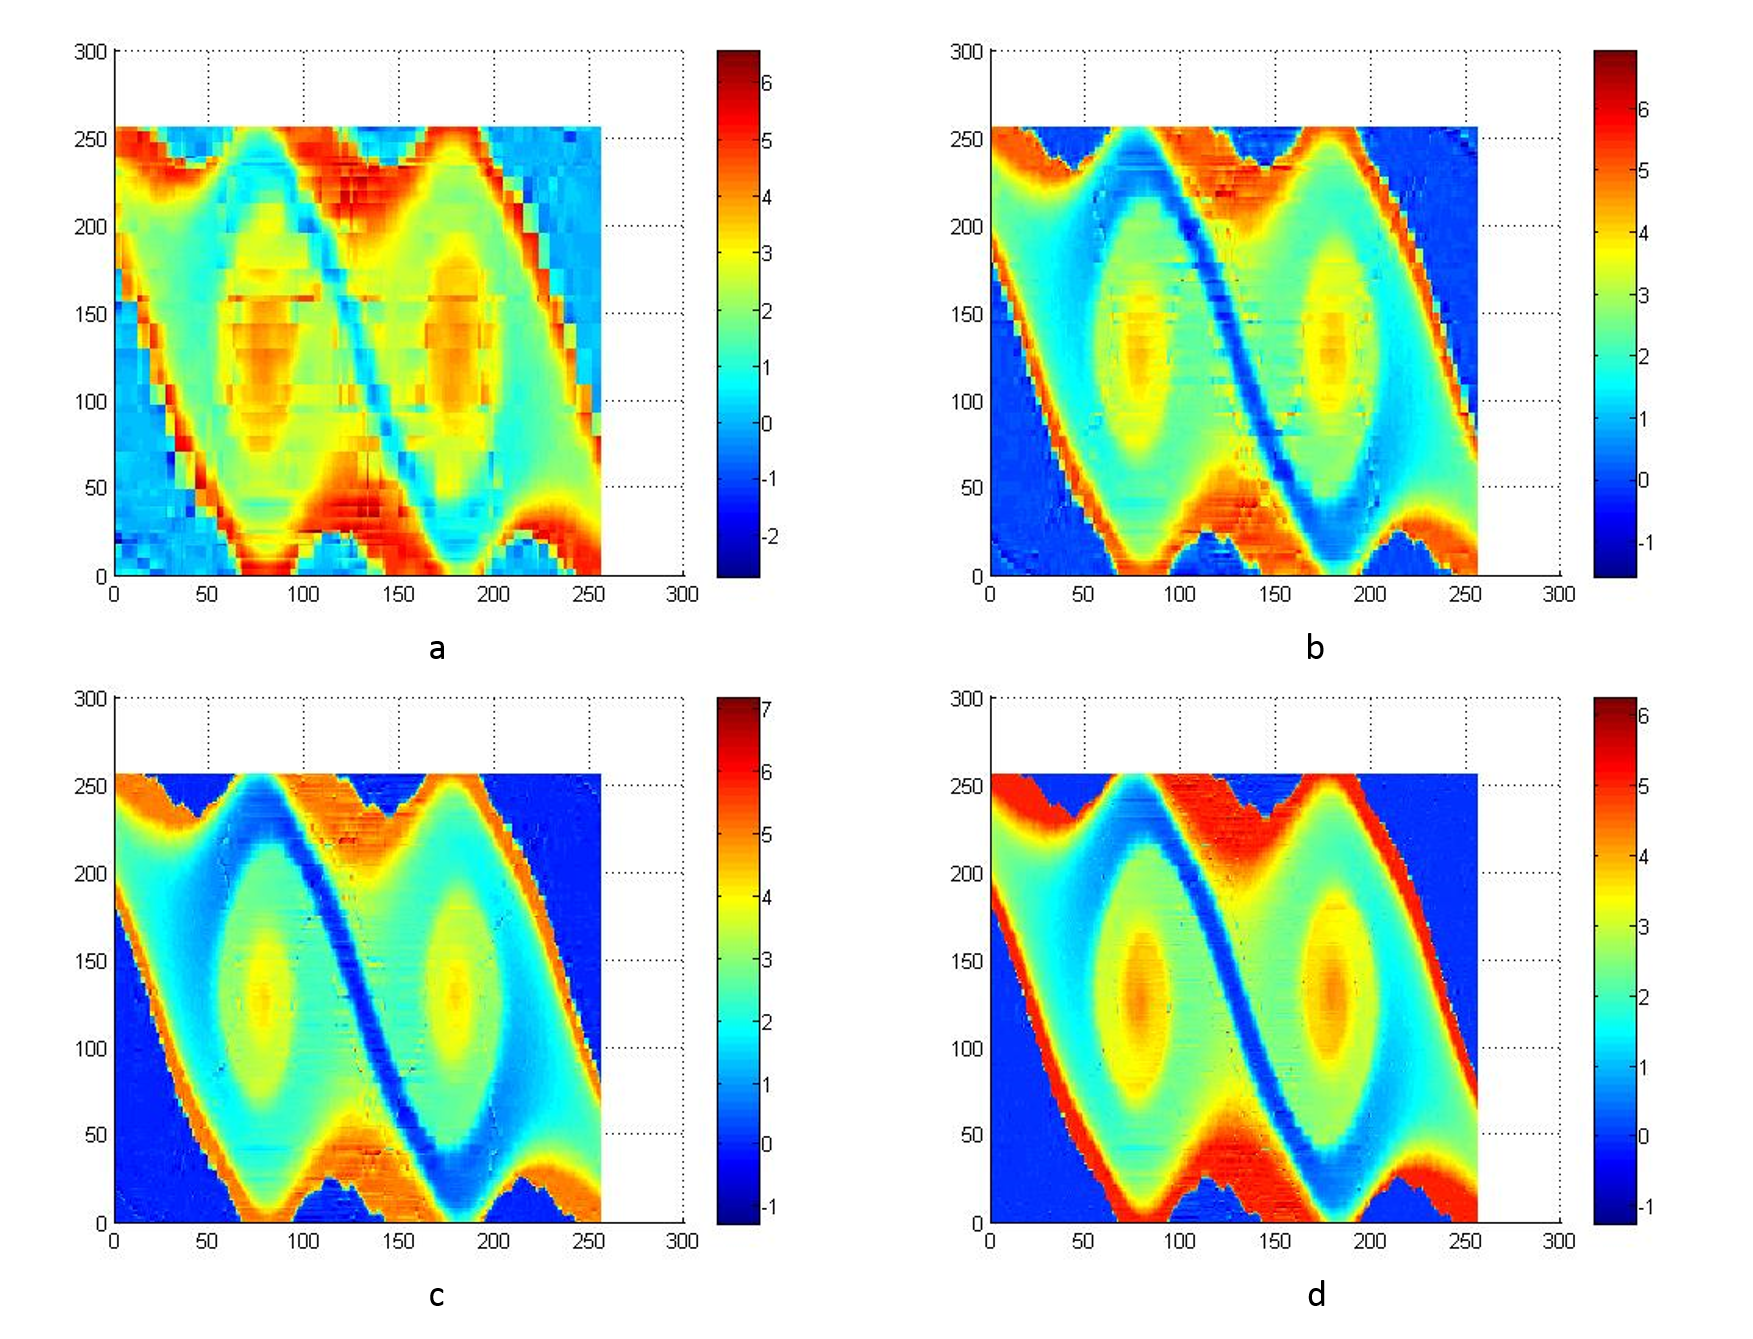
\includegraphics[scale=0.3]{CUR_valuefunctions}
		\caption{Plot der Wertefunktion bei einer Auswahl von 20 (a) 50 (b) 80 (c) und 120 (d) Spalten und Zeilen bei einer 256x256-Matrix}
	\end{figure}
	\newpage
	Für die numerische Betrachtung ist es natürlich von unbestreitbarem Interesse zu wissen, wo die größten 
	Fehler vorkommen. Im Falle, dass die größten Fehler vor allem am Rand des stabilisierbaren Bereiches auftreten 
	und im Inneren der Matrix gilt, dass $V_{CUR}\approx V_\mathcal{P}$, so können die Fehler am Rand 
	vernachlässigt und eine ungenauere Approximation verwendet werden. 
	\begin{figure}[h]
		\center
		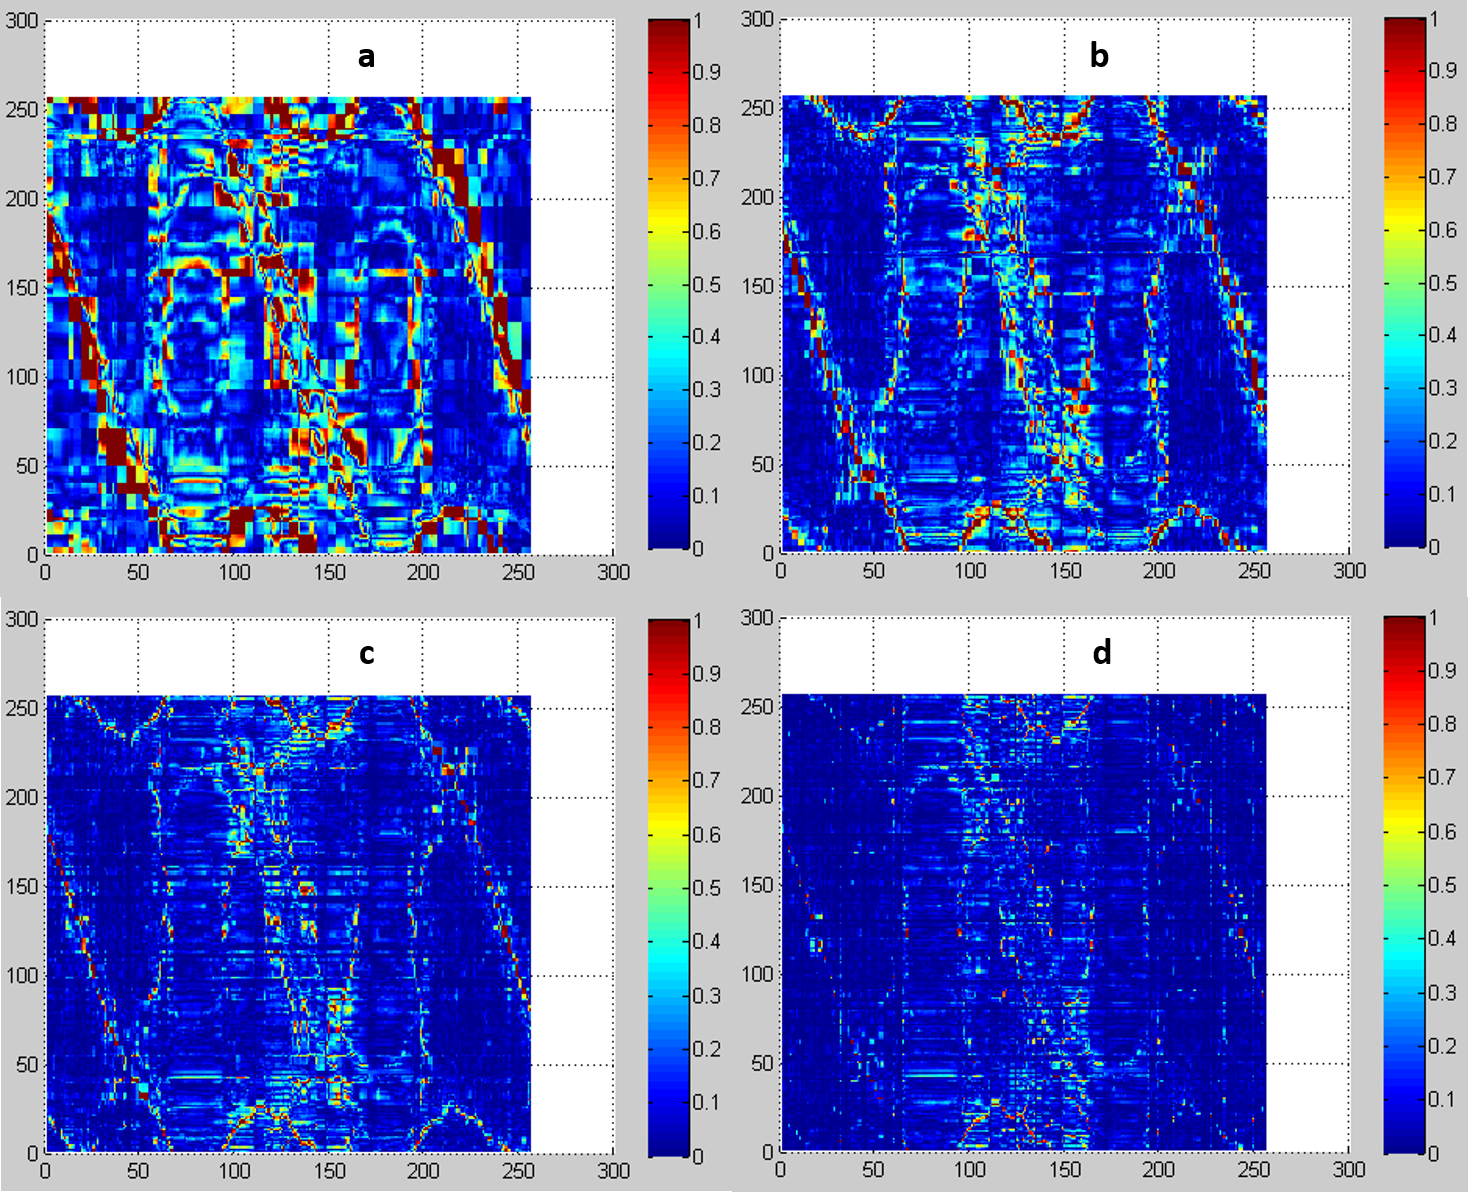
\includegraphics[scale=0.3]{CUR_fehlerstellen}
		\caption{Lokalisierung der Stellen der größen Fehler der Wertefunktion bei einer Auswahl von 20 (a) 50 (b) 80 (c) und 120 (d) Spalten und Zeilen bei einer 256x256-Matrix. Zur besseren Übersichtlichkeit wurde die angezeigte Skala auf 0-1 eingeschränkt}
	\end{figure}
	\newpage

\section{Ausblick und Diskussion/Fazit}
	In dieser Arbeit wurden verschiedene Approximationsmethoden vorgestellt und angewandt. Für ein besseres Ergebnis bei der Berechnung des Residuums könnte es hilfreich sein, die CUR-Zerlegung auf nicht-negative Matrizen $U$ einzuschränken. Hilfreiche Arbeiten in diesem Bereich könnten u.A. Hyvönen et al. \citep{NNCUR} liefern.
	\end{comment}
	\newpage
\section*{Abkürzungen}
	\begin{tabular}{ll}
		i.i.d & unabhängig identisch verteilt \\
		m.h.W & mit hoher Wahrscheinlichkeit\\
		SVD & Singulärwertzerlegung \\
	\end{tabular}
	\newpage
\bibliography{BA_lib}
\end{document}
